\documentclass[10pt,a4paper]{article}
\usepackage[utf8]{inputenc}
\usepackage{amsmath}
\usepackage{amsfonts}
\usepackage{amssymb}
\usepackage{graphicx}
\usepackage{color}
\usepackage{float}

\usepackage{eurosym}
 
\usepackage{fancyhdr}
 
\pagestyle{fancy}
\fancyhf{}
\rhead{Amsterdam university of applied sciences}
\lhead{Swarming: Research}
\rfoot{Page \thepage}

\definecolor{codegreen}{rgb}{0,0.6,0}
\definecolor{codegray}{rgb}{0.5,0.5,0.5}
\definecolor{codepurple}{rgb}{0.58,0,0.82}
\definecolor{backcolour}{rgb}{0.95,0.95,0.92}
\usepackage{listings}
\lstdefinestyle{cstyle}{
    backgroundcolor=\color{backcolour},   
    commentstyle=\color{codegreen},
    keywordstyle=\color{magenta},
    numberstyle=\tiny\color{codegray},
    stringstyle=\color{codepurple},
    basicstyle=\footnotesize,
    breakatwhitespace=false,         
    breaklines=true,                 
    captionpos=b,                    
    keepspaces=true,                 
    numbers=left,                    
    numbersep=5pt,                  
    showspaces=false,                
    showstringspaces=false,
    showtabs=false,                  
    tabsize=2
}
\graphicspath{ {./images/} }

\begin{document}
\begin{titlepage}
    \centering
    \vfill
    {\Large

    Swarming\\

   
    {\small Research document}\\
        
        \vskip2cm
        {\small M. van Wilgenburg, W. Mukhtar, E. van Splunter, M. Siekerman, T. Zaal and M. Visser}\\
    }    
    \vfill
%    \includegraphics[width=1\textwidth]{WireS4}
    
    \vfill
    \vfill
\end{titlepage}

\newpage

\listoffigures
\newpage

\listoftables
\newpage

\tableofcontents
\newpage


\section{Protocol}
\subsection{Hardware}

For the internal communication between the different systems there are multiple protocols to chose from to transmit data. every subsystem with a microcontroller should be able to communicate with the rest of the system. Because every system should be able to share their information it is necessary to have a multimaster system which allows every system to share their information without being dependent on a single master. To see which protocols are viable multiple protocols will be compared.

Building a modular robot consisting of subsystems, there must be a method to let these "\textit{subsystems}" communicate with each other to exchange relevant information. 

Every subsystem features a micro-controller which must be capable of transmitting and receiving data.  

\subsubsection{TWI}
The name TWI stands for "Two wire interface" which strongly resembles Phillps' protocol $I^(2)C$. Like the name suggests the bus is build up using two wires, one is used for the clock signal and the other is used for the data signal. Each of these wires is connected to the powerline through a pull-up resistor so every subsystem connected to the line can pull the line down which other systems can see. TWI can be used as a multimaster system which means every subsystem can send it's data without being dependend on a single master.

\begin{figure}[H]
        \centering
        \graphicspath{ {./images/} }
        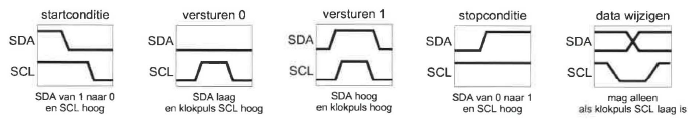
\includegraphics[scale=.6]{datacondities}
        \caption{Data conditions}
        \label{fig:Data conditions}
\end{figure}
In the above figure multiple data and clock combinations are shown, these combinations define the message start, sending a zero, a one and a stopbit. The system that wants to send information starts a message bij changing the datasignal from one to zero on a high clocksignal. All systems that are listening now know one of the systems is going to send a message. Data can be send by changing the dataline from zero to one or the other way around during a low clocksignal, the other systems will read this bit when the clocksignal becomes high again. Once the system is done sending its message it will let the other systems know by sending a stopbit.

\begin{figure}[H]
        \centering
        \graphicspath{ {./images/} }
        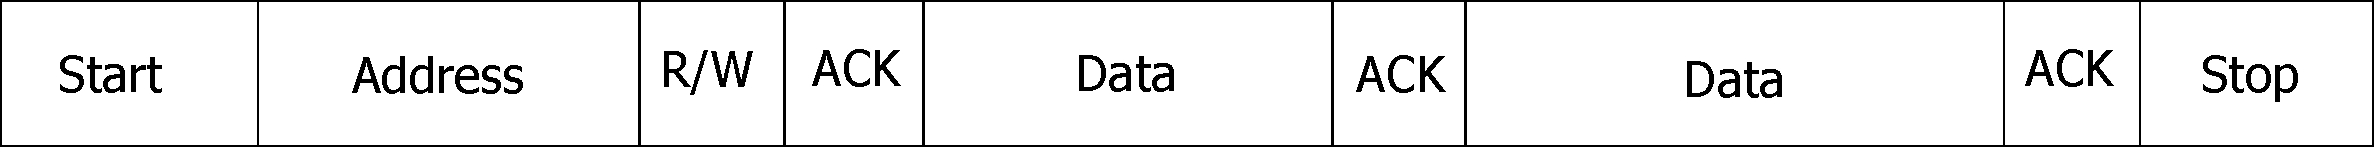
\includegraphics[scale=.6]{TWImessage}
        \caption{Structure of a TWI message}
        \label{fig:TWIstructure}
\end{figure}
In the above picture the structure of a message is shown. As explained before the message starts with a startbit after which a small header follows. The header contains information about who is going to be adressed by the message and if you want to read or write. After this the adressed system will respond with an acknowladge to make sure the information has come across. When the acknowladge is recieved the system will start sending data, followed by and acknowladge from the reciever after every recieved byte of data. when the system is done sending all of its data and recieved the last acknowladge it will send the stopbit which means all communication has ended.
\\
\\
TWI has a few benefits, because it is a simple serial protocol it only uses two wires. this saves a lot of space in the hardware design. Also, it has the possibility to be used as a multimaster system.
The speed of the communication depend on the frequency of the controller that will be used.


\subsubsection{SPI}
SPI or Serial Peripheral Interface is, like it names suggests, a serial interface. This interface can be connected in two ways, each having its own advantage. How this works will be explained using the following figure.
% \begin{figure}[H]
%         \centering
%         \graphicspath{ {./images/} }
%         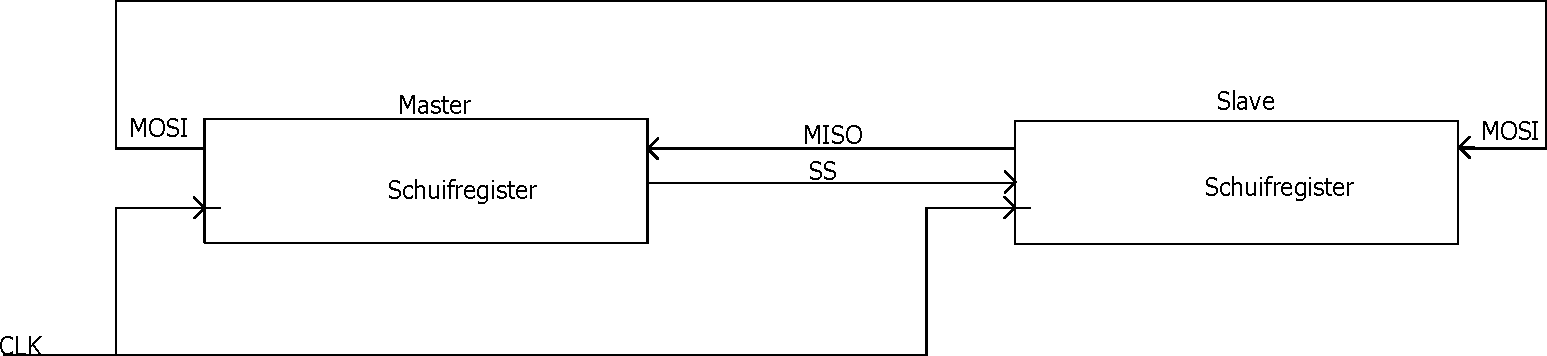
\includegraphics[scale=.6]{SPI}
%         \caption{SPI connections}
%         \label{fig:SPIconnections}
% \end{figure}

\subsubsection{UART}
\subsection{Software}


\newpage

\section{Relative Distance}
Building a swarm robots consisting of multiple units, location awareness may be required to ensure an more efficient operation. Implementing location awareness into a swarm of robots could result in better cooperation. For example: exploration based tasks can be executed on a much lower time scale. With location awareness the swarm can spread out evenly making sure that every part of the perimeter will be explored thoroughly. 

With location awareness it is also possible to divide the swarm into multiple groups. Because the location of every individual is available these individual groups can be formed very quickly by selecting the nearest unit. This also enables quick assists when an individual robot gets stuck or needs to execute a task that require more than one unit.

Relative distance can be measured in various ways using various methods. The most common methods are \textit{"Received Signal Strength Indication"} and \textit{"Time Of Flight"} abbreviated as RSSI and TOF. 

\subsection{Received Signal Strength}

\newpage

\section{Onderzoek}
Hier tekst plaatsen

\subsection{Propulsion,Actuators and Effectors}

In this chapter the sub-questions about the propulsion, actuators and effectors are researched and answered. First of all, the possible types of propulsion will be researched. Then the various kinds of actuators with a suitable effector will be considered. Depending on the situation different types of propulsion is used. For example a robot that operates in an environment with water would not be implemented with DC motor drivers and tyres. The robot build in this research should be able to operate on Mars in the future. Therefore the robot cant get stuck easily since that will cost millions, since the robot cannot complete his mission. Since swarming and not propulsion is the main goal of this research a simple way of locomotion would suffice. However there should be the possibility to implement a different kind of propulsion in the future, so that the robot can be used on Mars. 


%In dit hoofdstuk worden de deelvragen over de aandrijving, actuatoren en effectoren beantwoord. Allereerst zal er onderzocht worden welke soorten aandrijving er mogelijk zijn.Vervolgens zal er worden gekeken welke actuatoren er gebruikt kunnen worden en hoe de energie van de actuator gebruikt kan worden om de robot voort te bewegen. Als laatste wordt er gekeken welke effectoren nodig zijn. Robots worden op veel verschillende manier aangedreven, afhankelijk van de situatie.Bijvoorbeeld een robot die op het water moet opereren zal niet vaak met DC motoren met wielen worden ge\"implementeerd. In dit onderzoek kijken we naar een robot die in de toekomst mogelijk naar mars gestuurd kan worden. Dan kan de robot niet zomaar vast komen te zitten, aangezien er dan miljoenen voor niks verloren gaan. Omdat er eerst met een vereenvoudigde werkelijkheid wordt gewerkt is het vooral belangrijk dat de robot eenvoudig kan voortbewegen. Wel moet er ruimte zijn om later een andere module te kunnen aansluiten zodat hij ook op mars zich zou kunnen voortbewegen. 

\subsubsection{Effectors}
The way a robot moves is determined by its effector with his corresponding actuator. Possible types of effectors are:

%Door een effector aan een actuator de koppelen kan een robot zich voortbewegen. Mogelijke effectoren kunnen zijn:

\begin{itemize}
\item Wheels
\item Leg(s)
\item Catepillar tracks
\item Air cushion  
\item Propeller 
\item (Superconductor)
\end{itemize}

Each of these effectors have pro's and con's in different situations. Tyres are easily implemented, but there are various ways to implement these. The amount of tyres used will affect the handling of the robot. With a minimum two tyres, movement can already be realized. The downside is that driving with two wheels is not stable, only with algorithms that can balance the robot stable movement can be accomplished. It would be easier to implement more than two wheels so that the robot is more stable and movement is easier. 


  
%hier gebleven met vertalen
Elke van deze effectoren hebben voor en nadelen in verschillende situaties.\\Wielen zijn eenvoudig te implementeren, er kunnen verschillende aantallen wielen worden aangebracht. Het aantal wielen heeft wel invloed op het rijgedrag van de robot. Met twee wielen kan er worden gereden, mits de robot in balans wordt gehouden. Dit kan worden gedaan door middel van een zwenkwiel, of door een regelsysteem te bedenken dat de twee wielen de robot in balans houden. Dit laatste kost veel energie en is niet eenvoudig. Met drie wielen staat de robot al een stuk stabieler. Het nadeel hiervan is dat sturen soms moeizaam kan zijn. Met vier wielen is de robot nog stabieler en kan er op verschillende manieren worden gestuurd. De wielen kunnen tegengesteld worden aangedreven waardoor de robot draait. Dit kost wel meer energie dan nodig is aangezien er extra wrijving ontstaat. Een optie is de voorste wielen te laten draaien, waardoor de robot in de richting van de wielen zal voortbewegen. Zoals bij een auto het geval is. Dit is weer lastiger te implementeren aangezien er een soort van stuurmechanisme moet worden bedacht. 

\subsubsection{Actuatoren}

De keuze van de actuator hangt sterk samen met de effectoren.

\subsubsection{Aandrijving}

\newpage
\section{Swarm Communication}
There are several requirements to realise a robot swarm. Each member of the population needs to communicate with the rest of the swarm. To give the members full freedom of movement the communication also needs to be wireless. It is important that the population size of the swarm is dynamic, because of the scalability of the swarm. As mentioned earlier a swarm does not have a master. So each member needs to be capable to maintain the network. These networks also must be able to reroute around nodes that have been lost.

To create an network with those characteristics a (wireless) mesh network ((W)MN) is a possible solution. A mesh network relies on communication nodes in which data is distributed. All of the communication nodes cooperate in the distribution of data in the network. Each node of the network is connected to one or more nearby in range node(s) and forwards data on behalf of the other nodes. \cite{meshnetworking} A example of an mesh network is illustrated in figure \ref{fig:WMN}. To ensure a realiable network, self-organization and topology control alogorithms are needed.\cite{WMN1} Mesh networks can use self-healing algorithms such as Shortest Path Bridging (SPB) to restore and reroute the connection around broken nodes/clients. Shortest path bridging calculates the most favorable connections to the clients with the lowest path costs. \cite{SPB} Other usefull algorithms are listed in \cite{position-based}. The most efficient algorithm for path bridging depends on the situation where the clients are operating in which is described in \cite{position-based}.

A wireless mesh network (WMN) is a dynamically self-organized and configured network. \cite{WMN1} Each node or client in the network is able to create an ad hoc network to maintain the mesh connectivity, this is called client WMN's. These networks are able to reroute around nodes that have been lost. On large scale projects wireless mesh networks are costefficient because of the saving of wired connections.\cite{meshnetworking}

\begin{figure}[H]
   \centering
   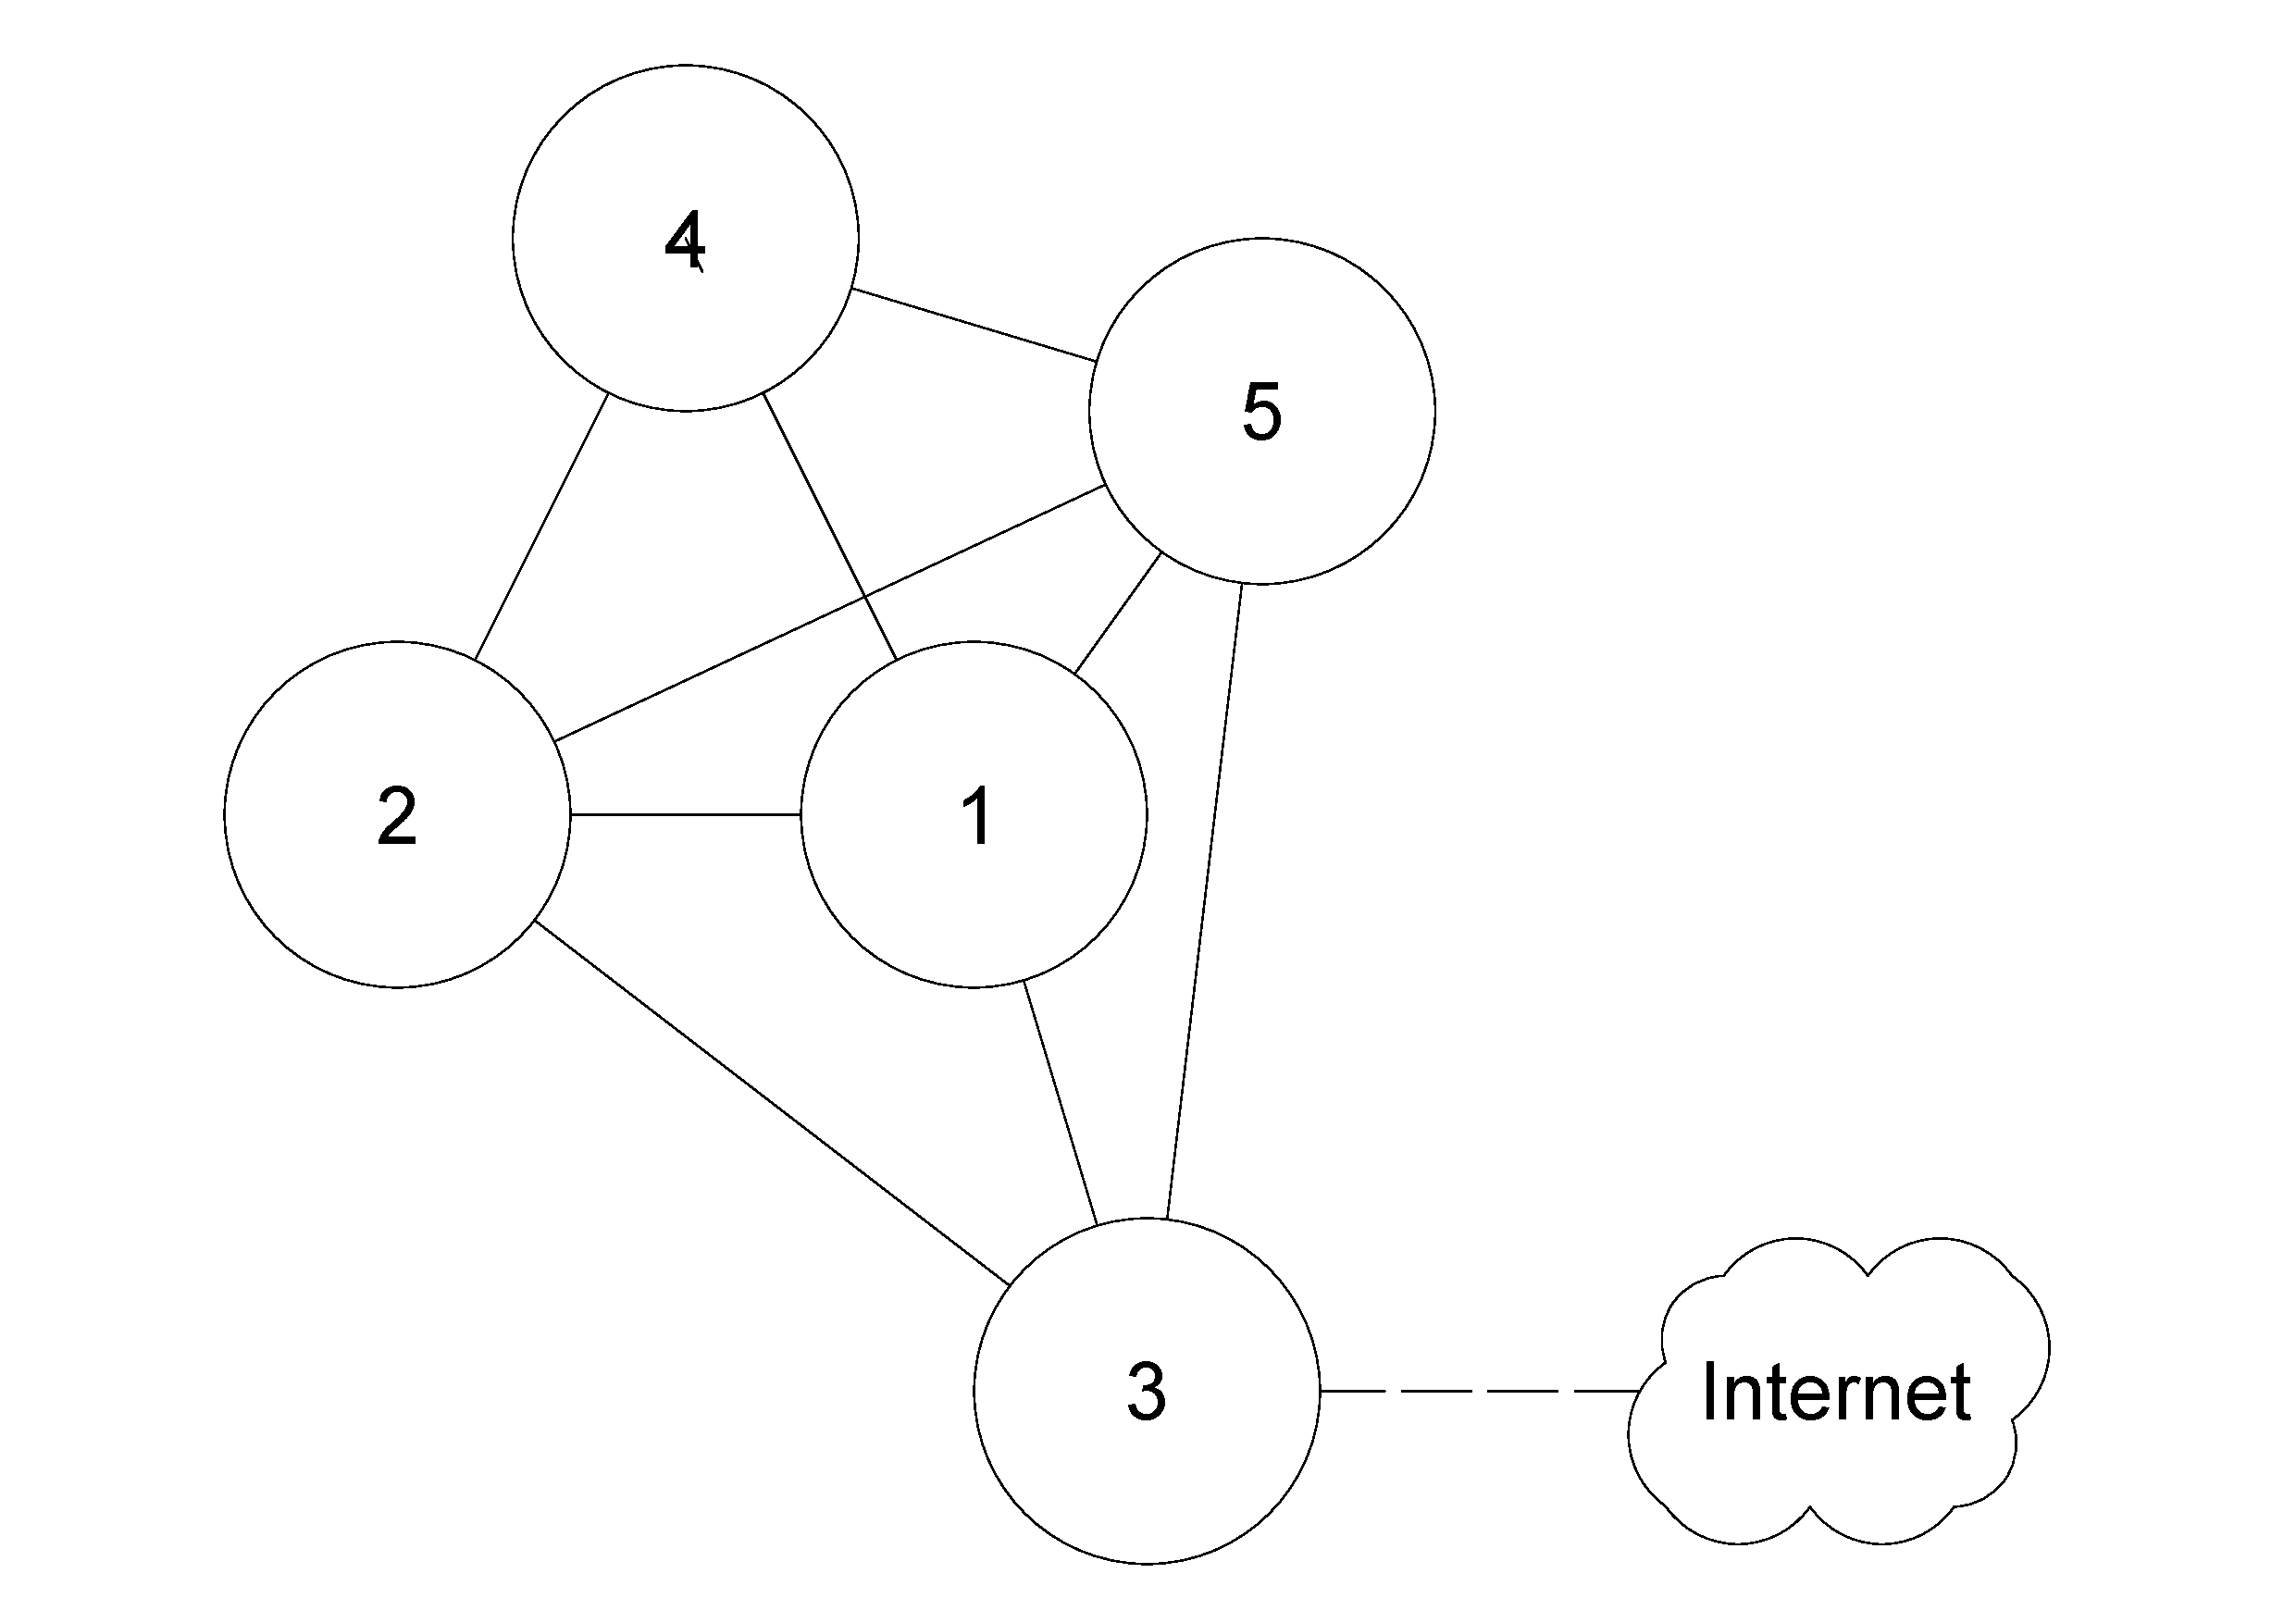
\includegraphics[width=1\textwidth]{WMN}
   \caption{An example of a wireless mesh network with 5 clients and an optional internet connection. The connections made in this example are random.}
   \label{fig:WMN}
\end{figure}




There exist several techniques to accomplish this method 
Examples of possible protocols:

% \begin{itemize}[noitemsep]
%     \item IEEE 802.11
%     \item ZigBee
%     \item SwarmBee
% \end{itemize}

\newpage




For close range obstacle avoidance, the robots will need some kind of proximity sensing technique. The sensor needs to differentiate between different "treats" for the robot to function properly. For example; when the sensor detects a small hill, which the robot can move over it should not trigger the robot to move away from it. But when it detects a big obstacle it should trigger the robot to move away. This is important because the robots will eventually be expected to move across rough terrain (like Mars). In the next paragraphs some different proximity sensor techniques will be discussed. Price is also a important factor while comparing these techniques. Multiple robots must be made on a tight budget, so costs should be cut where possible.\\


\subsubsection{Ultrasoon sensor}
Een veel gebruikte proximity sensor op simpele robots is de ultrasoonsensor. Dit komt omdat deze in vergelijking tot andere sensoren een goedkope oplossing is. Een ultrasoon sensor stuurt een ultrasoon geluid uit dit geluid wordt teruggekaatst tegen het object en vervolgens weer opgevangen door de sensor. De tijd die het geluid er over gedaan heeft wordt gemeten. Met een simpel rekensommetje wordt vervolgens de afstand bepaald. Een probleem met de ultrasoon sensor is dat het moeilijk is om te discrimineren tussen verschillende objecten. Hierdoor wordt het moeilijk om onderscheid te maken tussen bijvoorbeeld een heuveltje (waar de robot wel overheen kan) en een obstakel die de robot moet ontwijken. Door de atmosfeer op mars wordt geluid ernstig gedempt hierdoor is ultrasoon niet implementeerbaar op mars \cite{soundonmars}. Voor testen op aarde is het echter wel een goed werkend en bewezen techniek.

\subsubsection{Lidar sensor}
Lidar staat voor “Light detection and ranging”. Deze sensor werkt volgens het zelfde principe als de ultrasoon sensor. Het is al bewezen dat de lidar techniek werkt op Mars. Met de Phoenix missie is er een lidar systeem gebruikt om wolken en atmosferische stof te meten\cite{lidarmars}. Het licht van de laser kon wolken meten op meerdere kilometers hoogte. Omdat licht zich zeer snel verplaatst, moet de elektronica in een lidar sensor ook snel zijn. Hierdoor is de prijs in vergelijking tot de ultrasoon sensor hoog.

\begin{figure}[!ht]

  \centering
      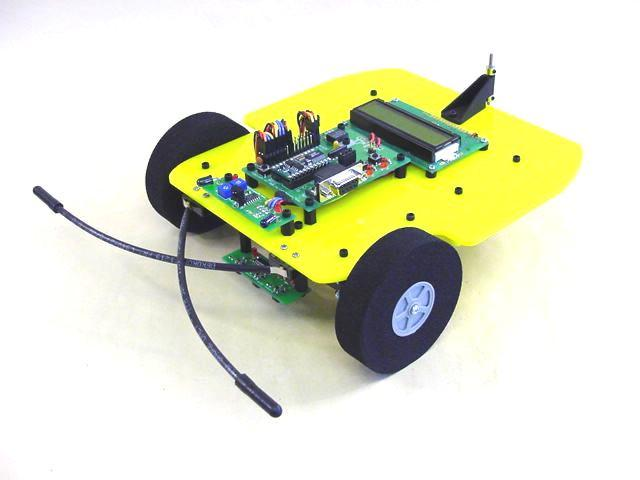
\includegraphics[width=0.5\textwidth]{voelsprieten.jpg}
  \caption{Robot met mechanische proximity sensor}  \label{voelspriet}
 
\end{figure}

\subsubsection{Mechanische sensor}
Eén mechanische proximity sensor bestaat meestal uit twee onderdelen. Dit zijn de actuator, dit is meestal een simpele druk schakelaar. En de arm of "bumper", dit is het deel dat het object aanstoot en zorgt dat de mechanishe kracht op de schakelaar wordt uitgeoefend figuur \ref{voelspriet} . De kracht van deze techniek is zijn eenvoudigheid. Er hoeven geen ingewikkelde signalen verwerkt te worden, enkel het aan of uit signaal van de actuator. Een groot nadeel van deze techniek is dat de sensor fysiek tegen een object aan moet komen om het te detecteren. In een zwerm van relatief fragiele robots is dit niet ideaal. Wanneer de robots zich op ruiger terrein bevinden, zal het gebruik van een "bumper" of arm ook niet ideaal zijn, deze kan namelijk vast blijven zitten tegen of achter obstakels.



\subsubsection{Sensor choice for the robot}
Now the question is which of the different sensor techniques proposed, is the best to implement on the swarm robots. While answering this question the following points will be taken into account:

\begin{itemize}
    \item The sensor must be easy to reproduce because multiple robots must be made from the swarm.
    \item The budget is limited, therefore the sensor price should be cheap compared the the total price of one robot.
    \item Energy usage should be as low as possible to increase the operation time per robot.
    \item For budget reasons there has been chosen to not take into account if the sensor would work on Mars.
\end{itemize}

Looking at these points it becomes clear that the lidar sensor wouldn't be the best choice. It doesn't really have any outstanding pros compared to the other two techniques and it's much more expensive. Currently the cheapest lidar sensor would cost about 100$\euro$. The ultrasonic and mechanical sensor wouldn't cost more than a few Euro's. As talked about before the mechanical sensor has a few drawbacks compared to the ultrasonic sensor. For these reasons the ultrasonic sensor seems the best choice. The only issue left to solve is how to sense the difference between obstacles which the robot has to avoid, and things the robot doesn't have to avoid, but still might be detected by the sensor. This will be discussed in the next paragraph.

\subsubsection{Obstacle discrimination with an ultrasonic sensor}
An ultrasonic sensor is usually used to detect if there is some obstacle in the way. In this case there is made no difference made between a obstacle that the robot can move over, or a obstacle that should be avoided. For example: a small slope or hill might be detected as an obstacle, but in truth the robot can move over it. The robots developed for this program will eventually be able to cross harsh terrain. In this case the proximity sensor will need to discriminate between these situations. Working with ultrasonic waves there are multiple domains to work with. These are time, frequency and amplitude. Time is used to determine the distance between the object and the sensor. The change in frequency and/or amplitude contains information about the shape of the object\cite{ultraobject}. 
In the paper "Object recognition with ultrasonic sensor" is concluded 
that looking at the amplitude over time contains enough information to discriminate between object\cite{ultraobject}. The example is given of an object with separated surfaces of 3,5cm, the echo from the second surface will be delayed by 0,2msec relative to the echo from the first surface. This delay can be easily detected with a microprocessor. The reason looking at frequency isn't the first choice is because of the higher hardware requirements it would require to properly sample the signal. 
\\

\newpage

\section{Bibliografie}
\bibliography{references}
\bibliographystyle{IEEEtran}



\end{document}